\subsection{Approach}\label{chapter_Approach}

At this point, all basics about the quadrocopter itself, the existing MATLAB Simulink model and about state space controlling should be clear. This chapter deals with the main part of what was developped in this research paper. 

\begin{figure}
	\centering
		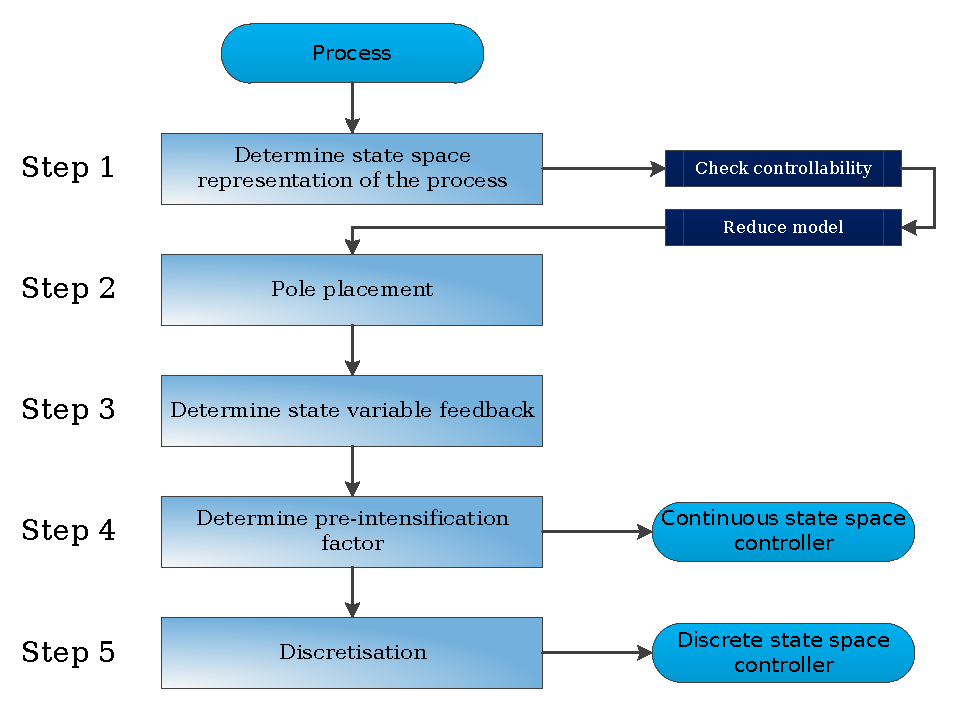
\includegraphics[width=1.00\textwidth]{03_Grafiken/Abstract.pdf}
	\caption{The five development steps}
	\label{fig:Abstract}
\end{figure}

To develop the state space controller the 'Five Steps', as they are named in the script of Prof.Kull (\cite{bib:KULL}), are used (figure \ref{fig:Abstract}). These steps are represented by the following sections. First step is to determine the state space representation of the process and check the controllability. Maybe it is necessary to reduce the model of the process. Thereafter, in the second step, the poles have to be placed in a wise order. In step three the state variable feedback factors for this specific pole constellation has to be calculated. Further on in step four, the corresponding pre-intensification factors must be estimated. After these four steps, the continuous state space controller for the MATLAB Simulink simulation and the basis for the implementation in C is completed. But to implement the controller into the quadrocopter - means in C - a discretization maybe is needed. The next chapter deals with that circumstance.

There are several reasons why MATLAB and MATLAB Simulink are used as development and simulation tool. One point is, that the cornerstone was implemented in MATLAB (chapter \ref{chapter_MATLAB_MODEL}). Another point is the uniqueness of MATLAB and MATLAB Simulink to combine all of the mentioned development steps in one tool. Even the HIL-Tests can be performed in this tool.
In the following sections the purpose, of why using MATLAB, will become clear.